\section{Halbleiteranwendungen}

\subsection{pn-Übergang und Bandstruktur}
	\begin{minipage}{0.5\linewidth}
		Als pn-Übergang wird die Kontaktstelle zwischen einem p- und n-dotiertem Halbleiter genannt. 
		Sobald der Kontakt entsteht, diffundieren die jeweiligen Majoritätsladungsträger auf die andere Seite. 
		Es entsteht die \textbf{Raumladungszone}, eine Zone, in der keine freien Ladungsträger veorhanden sind.
		
		\vspace{2mm}
		Inneres elektrisches Feld:
		
		$\boxed{E_0= -\dfrac{e N_A W_p}{\epsilon} = -\dfrac{e N_D W_n}{\epsilon}}$
		
		\vspace{2mm}
		Breite Raumladungszone:
		
		$\boxed{{W}_{0}=\sqrt{\dfrac{2\varepsilon \left({N}_{A}+{N}_{D}\right){V}_{0}}{e{N}_{A}{N}_{D}}} \sim \sqrt{V_0}} $
		
		\vspace{2mm}
		mehr Dotierung $\Rightarrow$ steilere Bänder
	\end{minipage}
	\hfill
	\begin{minipage}{0.5\linewidth}
		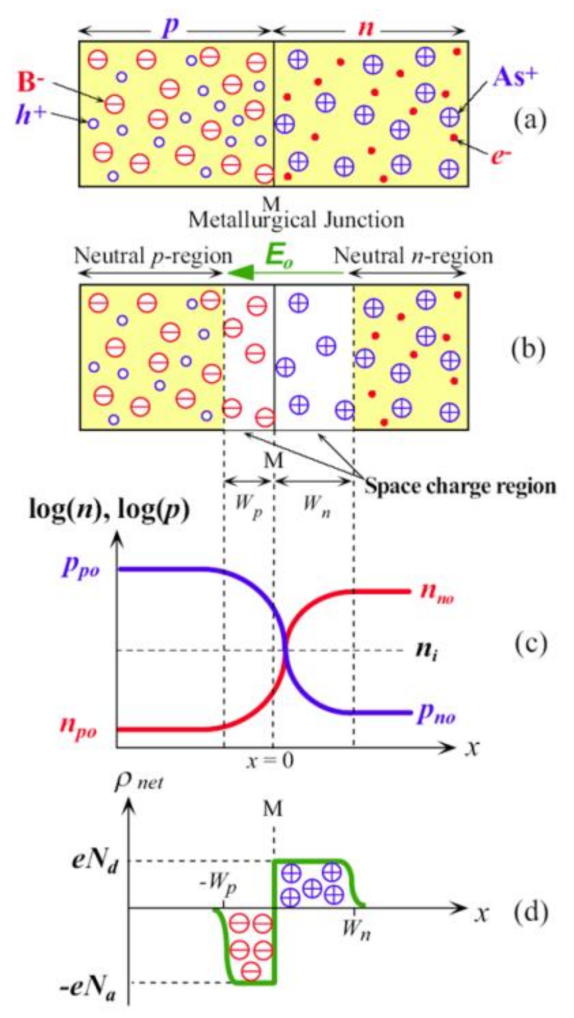
\includegraphics[width=0.85\linewidth]{Bilder/pn-Übergang}
	\end{minipage}

	\begin{minipage}{0.5\linewidth}
		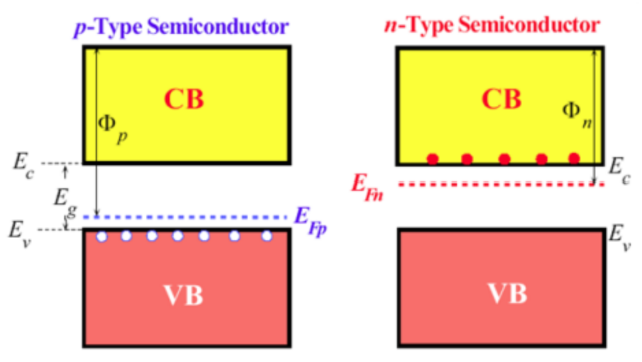
\includegraphics[width=0.99\linewidth]{Bilder/Bandstruktur_pn-Übergang-1}
	\end{minipage}
	\hfill
	\begin{minipage}{0.5\linewidth}
		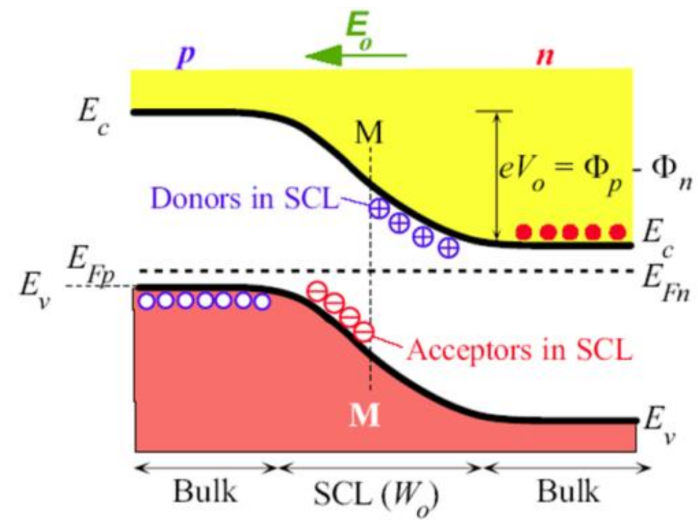
\includegraphics[width=0.99\linewidth]{Bilder/Bandstruktur_pn-Übergang-2}
	\end{minipage}
	
\subsection{Breakdown-Szenarien (beide können passieren)}
	\subsubsection{Avalanche-Breakdown}\label{Avalanche}
		\begin{minipage}{0.5\linewidth}
			Inneres elektrisches Feld \textbf{ionisiert!}

			\vspace{2mm}
			Bei kleinen Dotierungen dominant

			\vspace{2mm}
			$V_{breakdown} = $ Durchbruchspannung

			\vspace{2mm}
			$\dfrac{1}{M} = 1 - \left(\dfrac{\abs{V_r}}{V_{breakdown}}\right)$
		\end{minipage}
		\hfill
		\begin{minipage}{0.5\linewidth}
			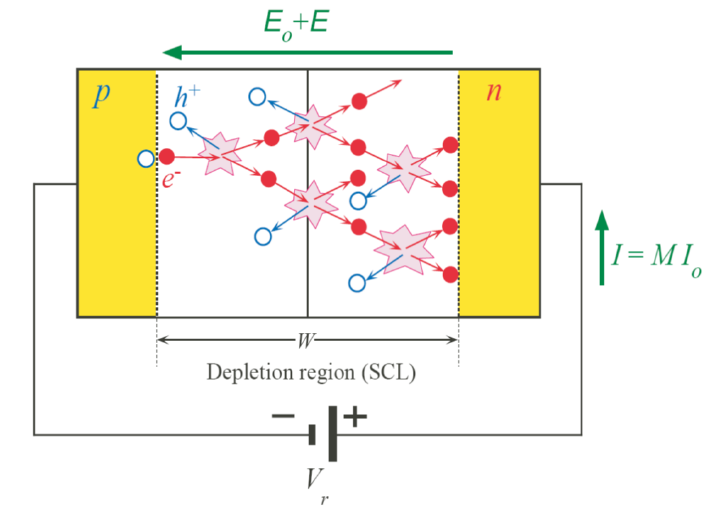
\includegraphics[width=0.9\linewidth]{Bilder/Avalanche-Breakdown}
		\end{minipage}

	\subsubsection{Zener-Breakdown (Tunneling)}
		\begin{minipage}{0.5\linewidth}
			Macht Übergang enger, stark gekrümmt

			\vspace{2mm}
			Bei starken Dotierungen dominant
		\end{minipage}
		\hfill
		\begin{minipage}{0.5\linewidth}
			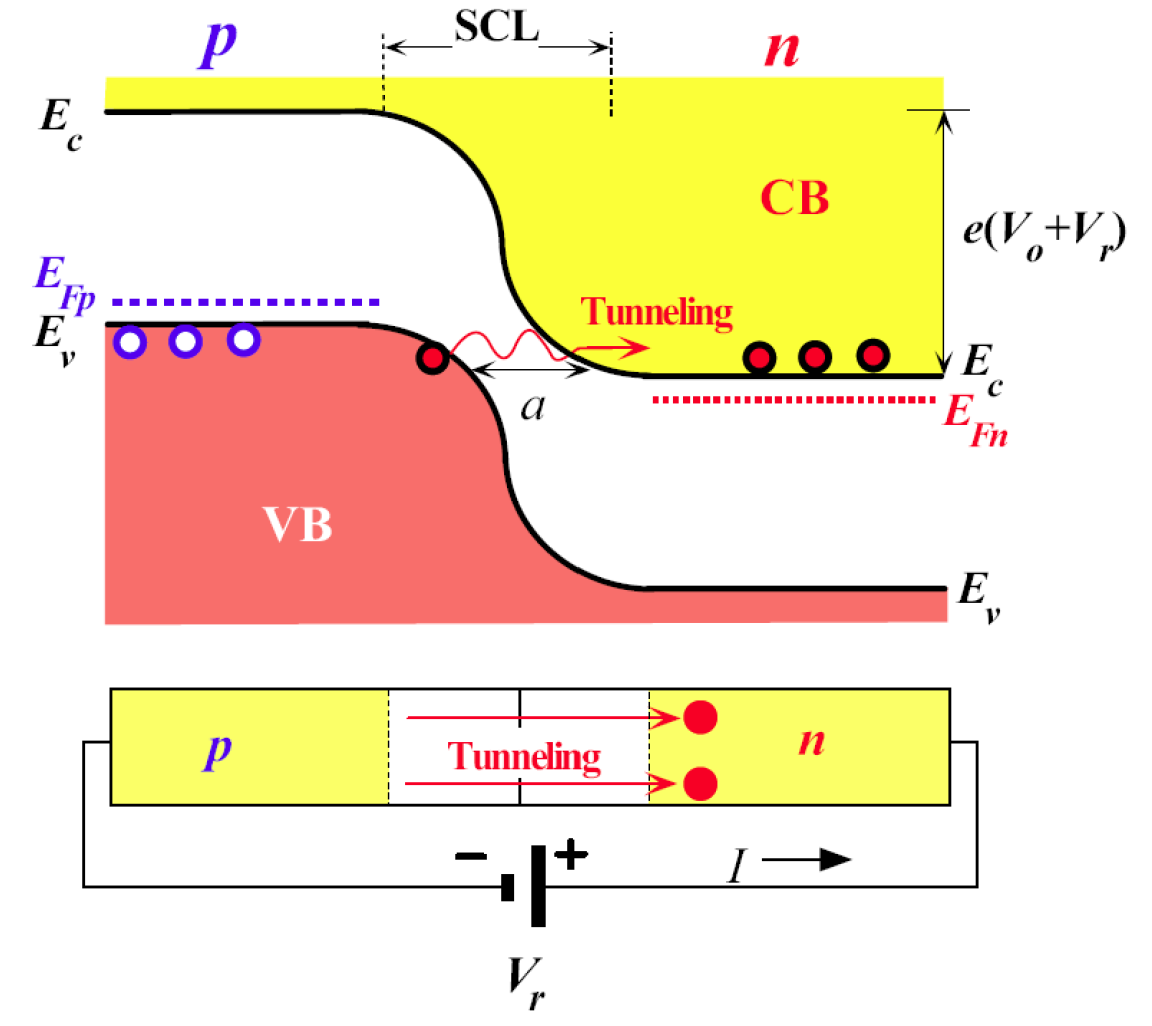
\includegraphics[width=0.9\linewidth]{Bilder/Zener-Breakdown}
		\end{minipage}

\subsection{Bipolarer Transistor: BJT}
	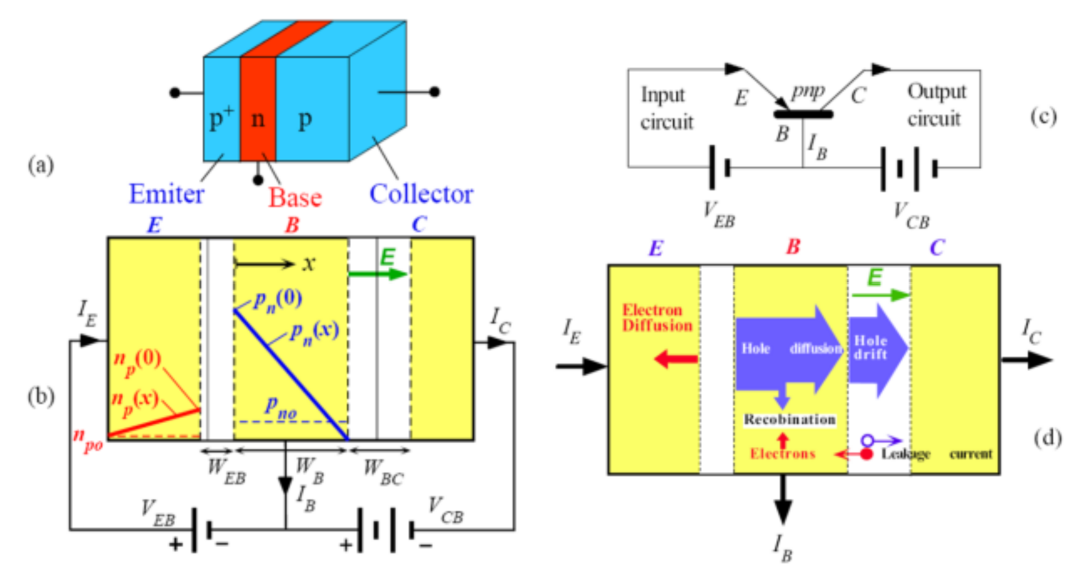
\includegraphics[width=0.9\linewidth]{Bilder/BJT}

	\begin{minipage}{0.5\linewidth}
		\begin{itemize}
			\item Regelung über $I_B$
			\item Kollektor saugt Löcher ab, da starkes inneres Feld
			\item Starke Dotierung im Emitter
		\end{itemize}
	\end{minipage}
	\hfill
	\begin{minipage}{0.5\linewidth}
		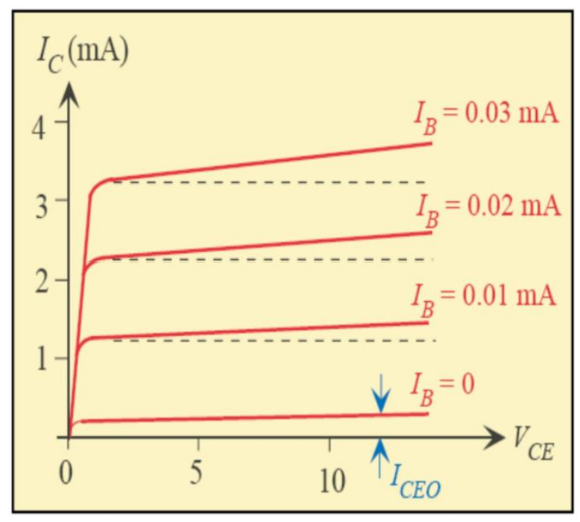
\includegraphics[width=0.8\linewidth]{Bilder/BJT-graph}
	\end{minipage}

\subsection{Sperrschicht-Feldeffekt-Transistor: JFET}
	\begin{center}
		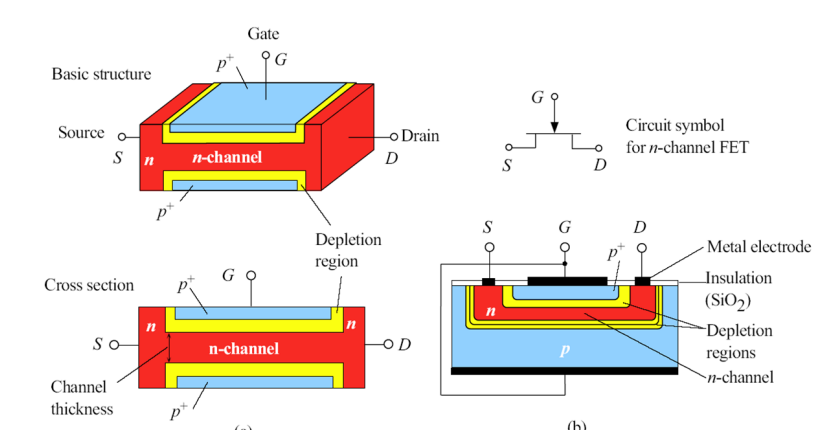
\includegraphics[width=0.8\linewidth]{Bilder/JFET_1}
	\end{center}

	\begin{minipage}{0.5\linewidth}
		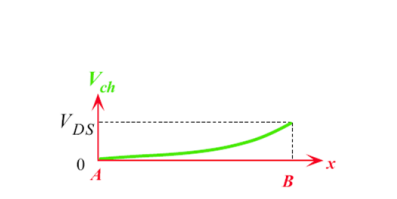
\includegraphics[width=0.8\linewidth]{Bilder/JFET_2}

		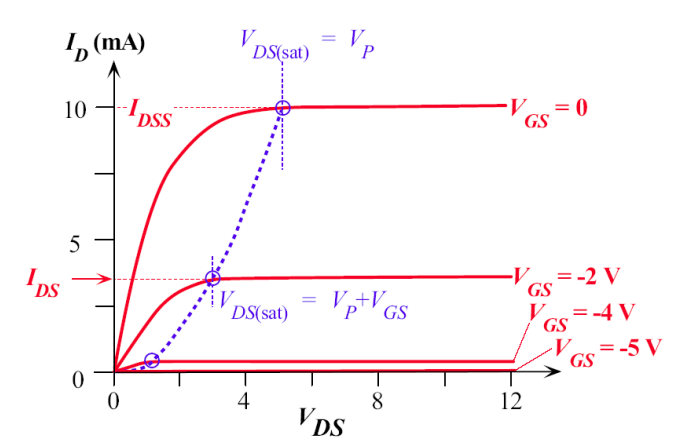
\includegraphics[width=0.99\linewidth]{Bilder/JFET_3}
	\end{minipage}
	\hfill
	\begin{minipage}{0.5\linewidth}
		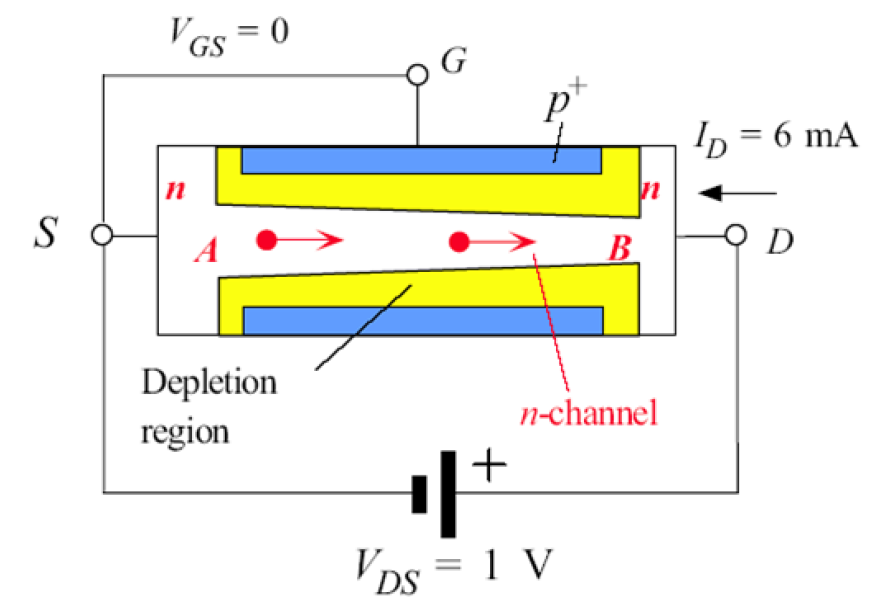
\includegraphics[width=0.8\linewidth]{Bilder/JFET_2a}

		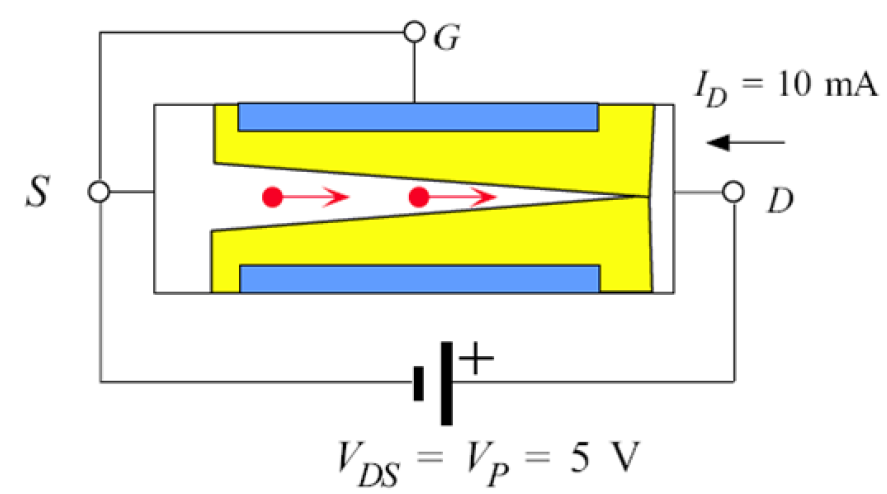
\includegraphics[width=0.8\linewidth]{Bilder/JFET_2b}

		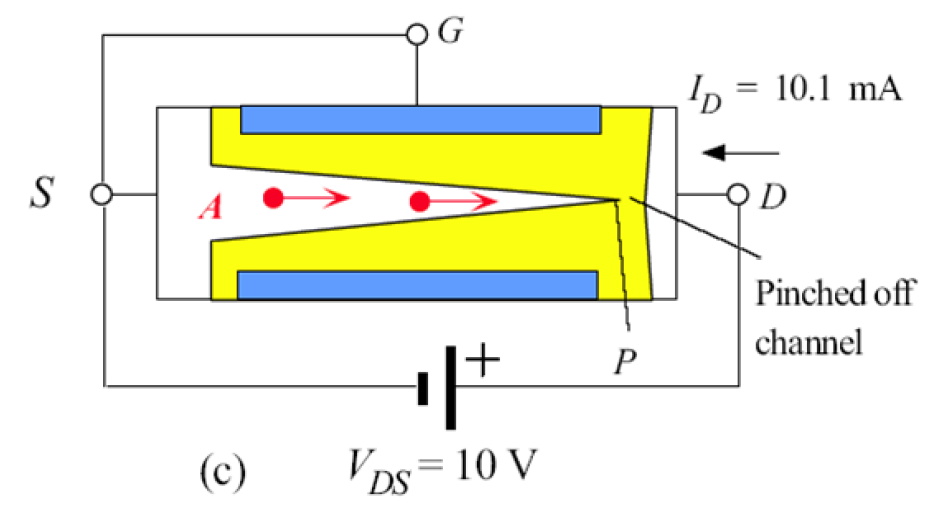
\includegraphics[width=0.8\linewidth]{Bilder/JFET_2c}
	\end{minipage}
	
	Wird eine negative Spannung zwischen Gate und Source angelegt, verengt sich der n-Kanal, 
	es fliesst weniger Strom und die Pinch-off Spannung wird reduziert.

	Wenn $V_{GS}$ klein genug ist, gibt es keinen n-Kanal mehr. 

	Es gibt aber trotzdem einen kleinen Stromfluss aufgrund von Leckströmen durch thermisch erzeugte Ladungsträger in der Verarmungsschicht.

\subsection{Metall-Oxid-Halbleiter-Feldeffekt-Transistor: MOSFET}
	MOS ist ein Metall-Isolator-Halbleiterübergang.

	\begin{minipage}{0.5\linewidth}
		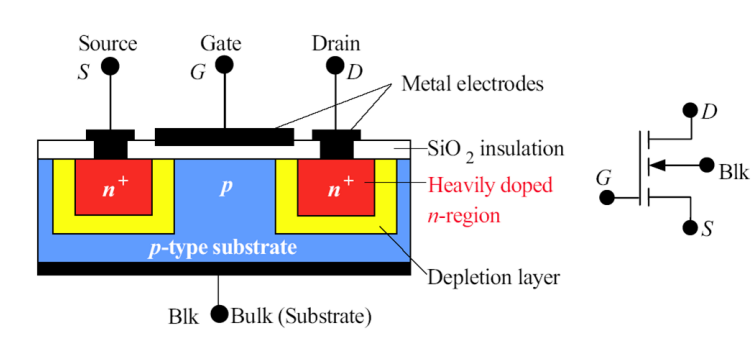
\includegraphics[width=0.99\linewidth]{Bilder/MOSFET_1}	
	\end{minipage}
	\hfill
	\begin{minipage}{0.5\linewidth}
		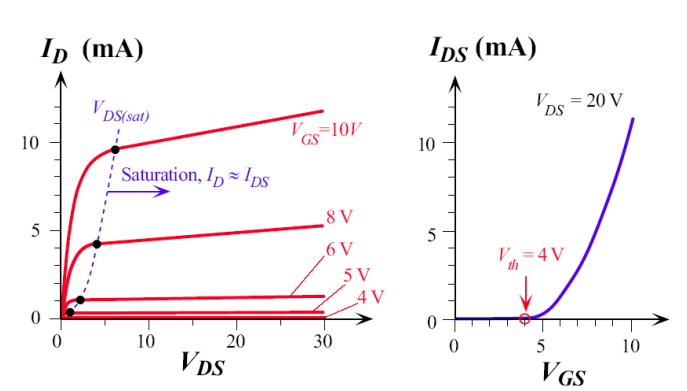
\includegraphics[width=0.99\linewidth]{Bilder/MOSFET_6}
	\end{minipage}

	\begin{minipage}{0.5\linewidth}
		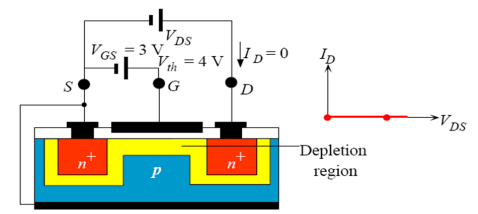
\includegraphics[width=0.99\linewidth]{Bilder/MOSFET_2}	

		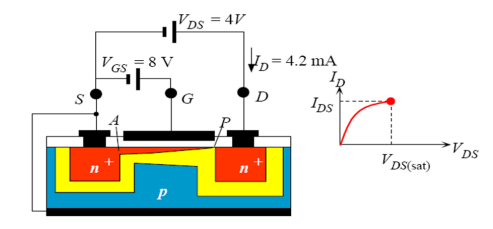
\includegraphics[width=0.99\linewidth]{Bilder/MOSFET_4}	
	\end{minipage}
	\hfill
	\begin{minipage}{0.5\linewidth}
		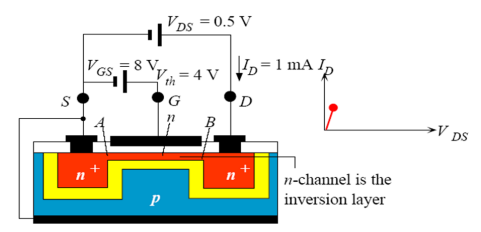
\includegraphics[width=0.99\linewidth]{Bilder/MOSFET_3}	

		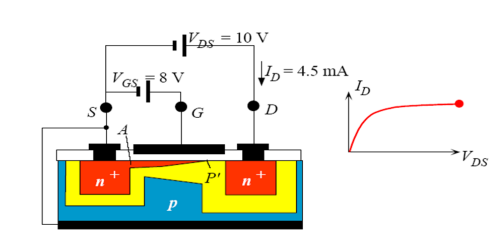
\includegraphics[width=0.99\linewidth]{Bilder/MOSFET_5}
	\end{minipage}
		
	Wird bei $V_{GS}$ eine Spannung angelegt, entsteht eine Verarmungszone im p-dot. Halbleiter.

	Sobald $V_{GS} > V_{threshold}$ bildet sich eine Inversionsschicht und 
	ein leitfähiger n-Kanal zwischen Source und Drain. Wird $V_{DS}$ erhöht, 
	bis zur Pinch-off Spannung oder weiter, fliesst kaum zusätzlicher Strom. 
	Die erhöhte Spannung erzeugt einen erhöhten Innenwiderstand, sodass der Strom begrenzt bleibt. 
	Der Strom $I_{DS}$ wird hauptsächlich von $V_{GS}$ bestimmt wird, siehe oben rechts.

\subsection{LED}
	\subsubsection{Funktionsprinzip}
		\begin{minipage}{0.65\linewidth}
			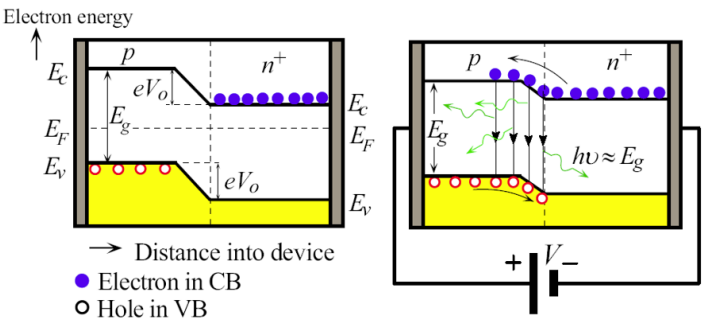
\includegraphics[width=0.99\linewidth]{Bilder/LED_1}
		\end{minipage}
		\hfill
		\begin{minipage}{0.35\linewidth}
			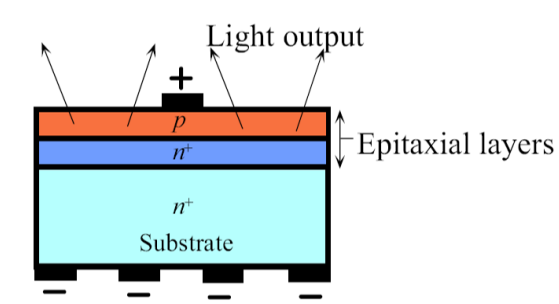
\includegraphics[width=0.99\linewidth]{Bilder/LED_2}
		\end{minipage}
		Die Potentialbarriere verhindert, dass Elektronen in den p-dotierten Bereich diffundieren, 
		wobei die Verarmungszone an der Grenze hauptsächlich im schwächer dotierten p-Bereich des pn-Übergangs anzutreffen ist. 
		Wird die Bias-Spannung nun erhöht, wird die Potentialbarriere verringert und die Elektronen und Löcher können diffundieren. 
		Durch die (erwünschte) Elektronen-Loch-Rekombinationsprozesse entstehen Photonen auf der p-dotierten Seite der Verbindung. 
		Diese Prozesse nennt man \textbf{induzierte Elektrolumineszens}. 
		
		Damit das Photon den Halbleiter verlassen kann, muss die p-dotierte Schicht \textbf{sehr dünn} sein.

\subsubsection{Heterostruktur fur Hochleistungs-LEDs}
	\begin{minipage}{0.6\linewidth}
		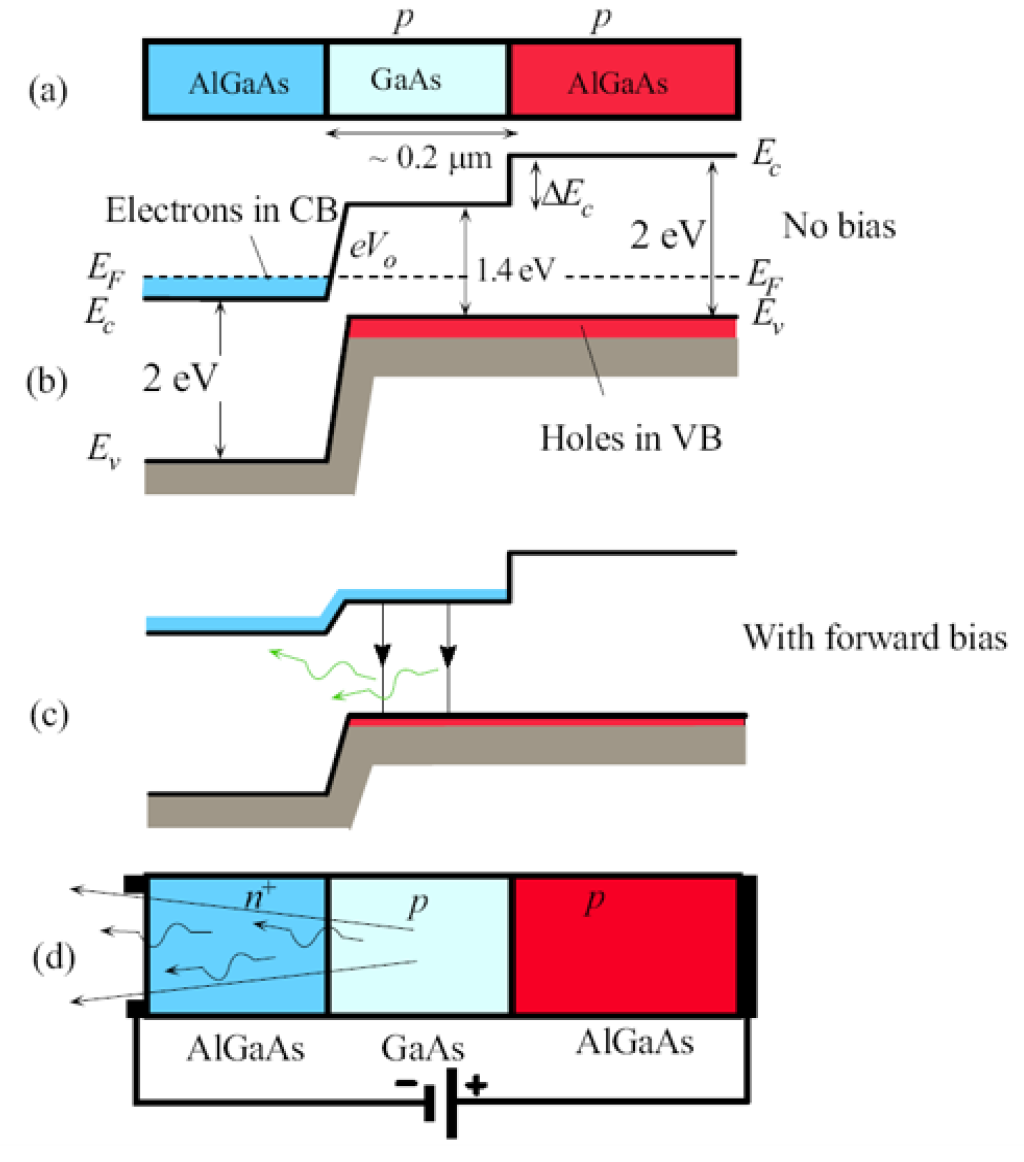
\includegraphics[width=0.99\linewidth]{Bilder/LED_3}
	\end{minipage}
	\hfill
	\begin{minipage}{0.39\linewidth}
		Durch die Verwendung verschiedener Halbleitern, einem Heteroübergang, 
		kann man die Eigenschaften einer LED deutlich verbessern.

		Links eine sogenannte Doppel-Heterostruktur. 

		Durch Anlegen einer Spannung gelangen die Elektronen ins Leitungsband der GaAs Schicht. 
		Sie werden dort aber durch die Potentialbarriere von AlGaAs aufgehalten. 
		Die Photonen können so gezielter freigesetzt werden. 
		Die Photonen, die in die falsche Richtung gehen, werden (anders als bei der normalen LED) 
		nicht absorbiert und können reflektiert werden.
	\end{minipage}

\subsection{Solarzelle}
\begin{minipage}{0.6\linewidth}
	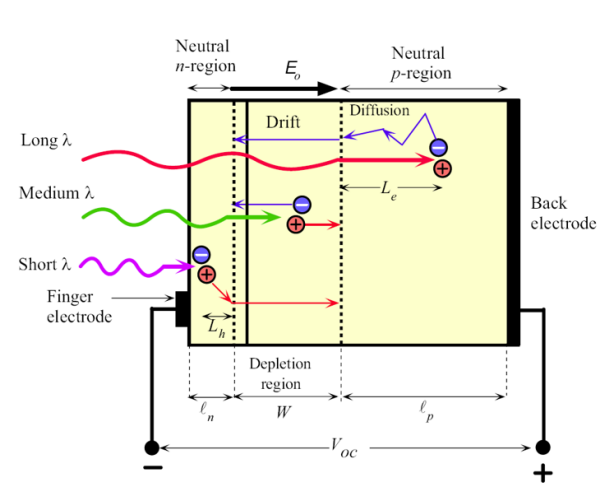
\includegraphics[width=0.99\linewidth]{Bilder/Solarzelle}
\end{minipage}
\hfill
\begin{minipage}{0.4\linewidth}
	Eine Solarzelle ist ein pn-Übergang, wobei der n-dotierte Bereich sehr dünn und transparent, aber stark dotiert ist.

	Die Photonen treten in dieser Schicht in den Halbleiter ein und erzeugen Elektronen-Loch-Paare. 
	Die Paare werden durch das innere elektrische Feld sofort getrennt und eine Spannung $V_{oc}$ entsteht.

	\[FF = \frac{V \cdot I}{V_{oc} \cdot I_{sc}}\]
\end{minipage}

\textbf{Il Fill Factor} misura quanto la caratteristica reale corrente-tensione di una cella solare 
si avvicini a un rettangolo ideale. Rappresenta il rapporto tra la potenza massima 
effettiva che la cella può erogare e la potenza teorica massima data dal prodotto 
della tensione a circuito aperto $V_{oc}$ e della corrente di corto circuito $I_{sc}$